%appendix
\chapter{Supplementary Material}

\section{Theory}

\begin{figure}
  \begin{tikzpicture}[
declare function={gamma(\z)=
2.506628274631*sqrt(1/\z)+ 0.20888568*(1/\z)^(1.5)+ 0.00870357*(1/\z)^(2.5)- (174.2106599*(1/\z)^(3.5))/25920- (715.6423511*(1/\z)^(4.5))/1244160)*exp((-ln(1/\z)-1)*\z;},
declare function={gammapdf(\x,\k,\theta) = 1/(\theta^\k)*1/(gamma(\k))*\x^(\k-1)*exp(-\x/\theta);}]
\begin{axis}[ymode=log, ymin=0,
no markers, domain=0:9, samples=100,
axis lines=left, xlabel=$\text{TS}$, ylabel=$\#\text{trials}$,
y label style={at={(axis description cs:-0.1,.5)},anchor=north},
x label style={dashed,at={(axis description cs:0.95,-0.1)},anchor=west},
height=5cm, width=9cm,
xtick={6,14.87}, ytick=\empty,
xticklabels={$\text{bg median}$,$5\sigma$},
%xticklabels={$\bar n (\theta_t)$},
enlargelimits=false, clip=false,% axis on top,
grid = major]
\addplot [very thick,cyan!20!black,domain=0:20, draw=none] {gammapdf(x,0.2,5)};
\addplot [very thick,cyan!20!black,domain=0.5:19.5] {gammapdf(x,0.2,5)};
%\addplot [domain= 0.5:4.5]{gauss(2.5,0.6,2)};
%\addplot [fill=cyan!20, draw=none, domain=0:6.0] {gammapdf(x,2,2)} \closedcycle;
%\addplot [very thick, fill=white!20!white, draw=none, domain=6.01:20] {gammapdf(x,2,2)} \closedcycle;
\end{axis}
\node at (2.5,1.7) {\begin{tikzpicture} \begin{axis}[hide axis,enlargelimits=false, ymax = 1,height=5cm, width=4cm,domain=2.65:3.35]\addplot [domain= 2.65:3.35,smooth,thick,green]{gauss(3,0.1,0.2)}; \end{axis} \end{tikzpicture}};
\node at (5.5,1.7) {\begin{tikzpicture} \begin{axis}[hide axis,enlargelimits=false, ymax = 1,height=5cm, width=3.5cm,domain=2.7:3.3]\addplot [domain= 2.7:3.3,smooth,thick,red]{gauss(3,0.07,0.14)}; \end{axis} \end{tikzpicture}};
\node[green] at (2.7,3) {$\xrightarrow{\text{90\%}}$};
\node[red] at (6,3) {$\xrightarrow{\text{50\%}}$};
\node at (0.5,3) {$\text{bg}$};
\node[green] at (2.7,4) {$\text{sensitivity}$};
\node[red] at (6,4) {$\text{discovery}$};
\end{tikzpicture}
\caption{Schematic showing the conditions to calculate the sensitivity and discovery potential. The background test statistic is shown in black, the signal test statistic satisfying the sensitivity conditions in green and the one for the discovery potential in red. Note that the curves dont actually look like these shown here. They have been simplified for explanatory purpose.}
\label{fig:sens_disc_schem}
\end{figure}

\section{Sources}

\begin{figure}
    \centering
    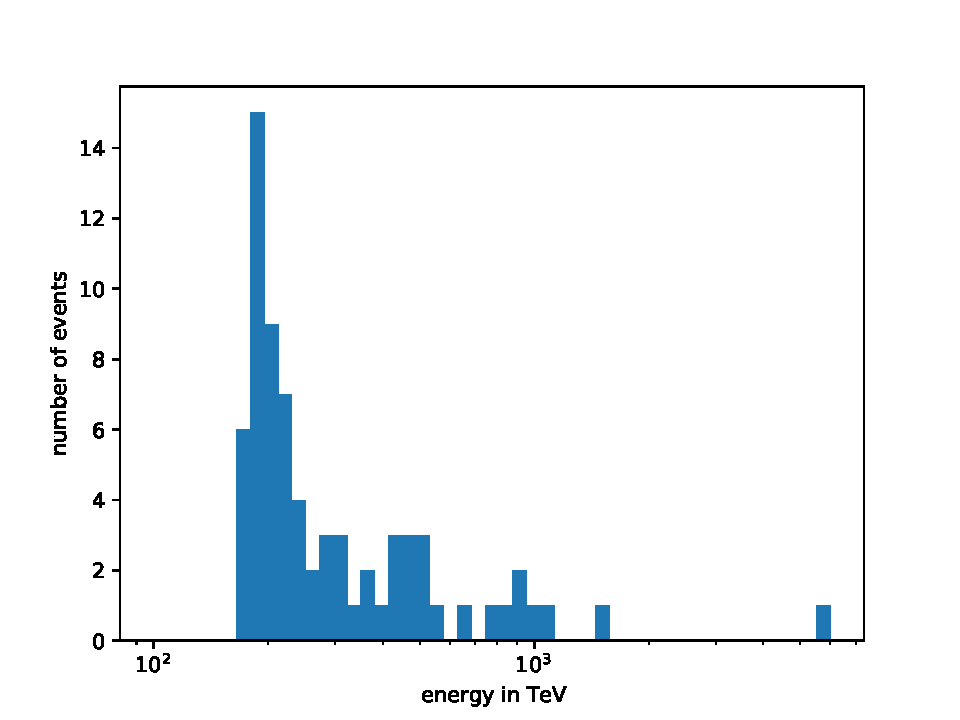
\includegraphics[width=\linewidth]{Plots/appendix/sources_energy.pdf}
    \caption{Histogram of the energy of the used sources seen in table \ref{tab:sources} in $\si{\tera\electronvolt}$.}
    \label{fig:sources_energy}
\end{figure}

\begin{table}
  \centering
  \caption{Table of the sources used in the time-dependent analysis. Additionally the signalness parameter is shown after which the sources were selected.}
  \label{tab:sources_time_dep}
  \begin{tabular}{ccrrc}
    \toprule
    Nr. & MJD &  $\delta$ in $\si{\degree}$ & $\alpha$ in $\si{\degree}$ & signalness in $\si{\percent}$ \\
    \toprule
      11 & 56819.20 & 11.45 & 110.65 & 99.70 \\ 12 & 56470.11 & 14.17 & 93.74 & 93.80 \\ 13 & 57951.82 & 25.16 & 208.39 & 86.60 \\ 16 & 58063.78 & 7.44 & 340.14 & 97.50 \\ 29 & 57340.87 & 12.71 & 76.16 & 95.70 \\ 37 & 55911.28 & 18.88 & 36.74 & 94.60 \\ 42 & 56226.60 & 27.91 & 169.80 & 92.60 \\ 43 & 56666.50 & 33.02 & 293.12 & 92.70 \\ 58 & 57478.57 & 15.48 & 151.22 & 85.10 \\ 63 & 56211.77 & -2.28 & 205.14 & 84.20 \\ 
    \toprule
  \end{tabular}
\end{table}

\section{Time-Integrated Search}

\begin{table}
  \centering
  \caption{Table of the number of injected signal events used for the time integrated analysis.}
  \label{tab:sig_time_int_table}
  \begin{tabular}{r}
    \toprule
    $n_\text{S}$ injected \\
    \toprule
      0.0 \\ 7.5 \\ 15.0 \\ 22.5 \\ 30.0 \\ 36.0 \\ 57.0 \\ 78.0 \\ 99.0 \\ 120.0 \\ 141.0 \\ 194.2 \\ 247.4 \\ 300.7 \\ 353.9 \\ 407.1 \\ 460.3 \\ 513.6 \\ 566.8 \\ 620.0 \\ 
    \toprule
  \end{tabular}
\end{table}

\begin{table}
  \caption{Table of the number of trials for each spectral index $\gamma$ and number of injected signal events $n_\text{sig}$, running $\num{10}$ jobs with $\num{5e4}$ trials per set of parameter pairs $\gamma$ and $n_\text{sig}$. Some jobs fail due to technical reasons.}
  \label{tab:trials_sig_time_int_table}
  \begin{subtable}{\linewidth}
  \centering
  \begin{tabular}{p{.9cm}|rrrrrrrrrr}
    \toprule
    \: $n_\text{sig}$ \newline $\gamma$ \: & 0.0 & 7.5 & 15.0 & 22.5 & 30.0 & 36.0 & 57.0 & 78.0 & 99.0 & 141.0 \\ 
    \toprule
    1.50 & 50000 & 50000 & 50000 & 50000 & 50000 & 50000 & 50000 & 50000 & 50000 & 50000 \\ 1.75 & 50000 & 50000 & 50000 & 50000 & 50000 & 50000 & 50000 & 50000 & 50000 & 50000 \\ 2.00 & 50000 & 50000 & 50000 & 50000 & 50000 & 50000 & 50000 & 50000 & 50000 & 50000 \\ 2.25 & 50000 & 45000 & 45000 & 45000 & 50000 & 45000 & 50000 & 50000 & 50000 & 50000 \\ 2.50 & 50000 & 50000 & 50000 & 50000 & 50000 & 50000 & 50000 & 50000 & 50000 & 50000 \\ 2.75 & 50000 & 50000 & 45000 & 45000 & 50000 & 50000 & 50000 & 40000 & 50000 & 40000 \\ 3.00 & 50000 & 50000 & 50000 & 50000 & 50000 & 45000 & 50000 & 50000 & 50000 & 50000 \\ 
    \toprule
  \end{tabular}
\end{subtable}
\begin{subtable}{\linewidth}
\centering
  \begin{tabular}{p{.9cm}|rrrrrrrrrr}
    \toprule
    \: $n_\text{sig}$ \newline $\gamma$ \: & 141.0 & 194.2 & 247.4 & 300.7 & 353.9 & 407.1 & 460.3 & 513.6 & 566.8 & 620.0 \\ 
    \toprule
    1.50 & 50000 & 50000 & 50000 & 50000 & 50000 & 50000 & 50000 & 50000 & 50000 & 50000 \\ 1.75 & 50000 & 50000 & 50000 & 50000 & 50000 & 50000 & 50000 & 50000 & 50000 & 45000 \\ 2.00 & 50000 & 50000 & 50000 & 50000 & 50000 & 50000 & 50000 & 50000 & 50000 & 50000 \\ 2.25 & 50000 & 50000 & 50000 & 50000 & 50000 & 50000 & 50000 & 50000 & 50000 & 50000 \\ 2.50 & 50000 & 50000 & 50000 & 50000 & 50000 & 50000 & 50000 & 50000 & 50000 & 40000 \\ 2.75 & 50000 & 50000 & 50000 & 50000 & 50000 & 50000 & 50000 & 50000 & 50000 & 50000 \\ 3.00 & 50000 & 50000 & 45000 & 50000 & 50000 & 50000 & 50000 & 50000 & 50000 & 50000 \\ 
    \toprule
  \end{tabular}
  \end{subtable}
\end{table}
